%%%%%%%%%%%%%%%%%%%%%%%%%%%%%%%%%%%%%%%%%%%%%%%%%%%%%
\chapter{Introduction} \label{chap:intro}
\graphicspath{{images/intro/}}

\gls{hri} what it is and what it matters and why it is challenging

Robots will inhabit human spaces and need to interact with them in decent ways

Robot behaviour unlikely to be programmable and static

This works explores how robots could interact with humans to learn from them to interact with other humans

%%%%%%%%%%%%%%%%%%%%%%%%%%%%%%%%%%%%%%%%%%%%%%%%%%%%%
\section{Scope}\label{sec:intro-scope}
\gls{hri} complex, definition of the the problem

\subsection{Frame}

robot not designed statically by engineers but entities which should be molded

teaching robot to interact with humans

assumption that some humans are experts in a domain that the robot have to learn
(could it be therapists, or simply a user being expert in knowing how they desire the robot to interact)

\subsection{Environment} \label{sec:scope-social}
Robot interacting in an environment shared with humans / directly with humans

human centred environment where the robot is supposed to complete a specific task

\subsection{Type of interaction}
Dyadic/Triadic interaction:
human expert + human target of the interaction

\begin{figure}[ht]
	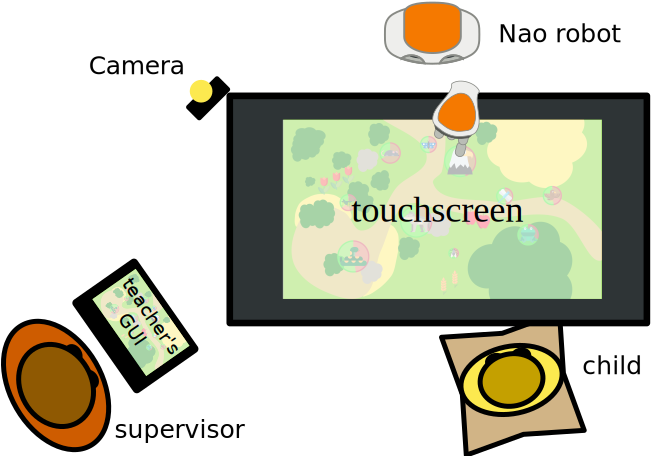
\includegraphics[width=.4\linewidth]{setup.pdf}
	\centering
	\caption{The setup used in the study: a child interacts with the robot tutor, with a large touchscreen sitting between them displaying the learning activity; a human teacher provides guidance to the robot through a tablet and monitors the robot's learning.}
	\label{fig:setup}
\end{figure}

\subsection{Algorithms}

different algo can be used to teach robot to interact:

\paragraph{Supervised Learning}

\paragraph{Reinforcement Learning}

Three different algorithms have been used in the progress of this research. The first study presented in Chapter \ref{chap:woz} uses feed forward neural network with a single hidden layer. the second study in Chapter \ref{chap:control} used \acrlong{rl} combining human and environmental rewards into a single reward source for the algorithm. And the last study presented in Chapter \ref{chap:tutoring} uses instance based algorithm adapted from Nearest Neighbours to enable quick and efficient learning. More details about each algorithms and their related work can be found in the associated chapters.

%%%%%%%%%%%%%%%%%%%%%%%%%%%%%%%%%%%%%%%%%%%%%%%%%%%%%
\section{The Thesis}\label{sec:intro-thesis}
The main thesis that this document seeks to put forward is as below.

A robot can learn how to interact meaningfully with humans by receiving supervision from a human teacher in control of the robot's behaviour, this supervision will lead to an efficient, safe and low human-workload teaching and autonomous behaviour.
%One sentence to describe the take home/conclusion

Additional research questions have been explored during the progress of this
work and are introduced here.

\begin{itemize}
    \item \textbf{What kind of interaction could allow a human to teach a robot to interact with other humans while ensuring an appropriate and adaptive interaction policy and a low workload on the human teacher?}
    
    	Justification for \gls{sparc} 
    \item \textbf{Does adding a learning component to a supervised robot can reduce the human-workload of the supervisor?}
    
        \gls{woz} is an approach widely used in \gls{hri} \citep{riek2012wizard}, whereby a human teleoperates a robot to have it interact with other humans. However, this method applies a high workload on the operator and is not scalable. Using \gls{ml} to learn from this operator online might decrease the operator's workload without decreasing the quality of the robot behaviour.
    
    \item \textbf{How control of a teacher over the robot's action impacts the robot's learning?} 
    
	    In the context of \gls{iml}, a human can provide inputs to an agent to speed up the learning. Other \gls{iml} \citep{thomaz2008teachable,knox2009interactively} focus on feedback from the human with limited or no control over the agent's actions. However increase the control should speed up the learning and reduce the number of errors made by the robot.

    \item \textbf{After receiving supervision from a human, could a robot behave autonomously in a social context?}

	 	\gls{sparc} has been designed to allow non-experts in \gls{ml} to teach agents how to interact while interacting. Human-robot interactions provide a perfect test for this approach: using a human to teach a robot how to behave in this complex and non-deterministic environment.
	 
\end{itemize}

%%%%%%%%%%%%%%%%%%%%%%%%%%%%%%%%%%%%%%%%%%%%%%%%%%%%%
\section{Approach and Experimentation}\label{sec:intro-exps}

introduction of structure, and especially why it is that way

why literature review, why and conclusion

how the results have been used to design a new interaction framework to teach robots to interact with humans

how it has been tested and why that order

%%%%%%%%%%%%%%%%%%%%%%%%%%%%%%%%%%%%%%%%%%%%%%%%%%%%%
\section{Key Concepts and terminology}\label{sec:intro-concepts}

Throughout this thesis, the terms `wizard', `supervisor' and `teacher' have been used interchangeably to represent the people in control of a robot's action and teaching that robot an action policy.

agent and robot

\begin{itemize}
	\item \textbf{Appropriateness}
	\item \textbf{Adaptivity}
	\item \textbf{Autonomy}
	\item \textbf{Supervised Autonomy}
	\item \textbf{Learning}
	\item \textbf{Teacher, wizard and supervisor}
	\item \textbf{Robot and agent}
\end{itemize}

%%%%%%%%%%%%%%%%%%%%%%%%%%%%%%%%%%%%%%%%%%%%%%%%%%%%%
\section{Challenges}

Complexity of interactions with humans: complex world, safety, workload and so on

%%%%%%%%%%%%%%%%%%%%%%%%%%%%%%%%%%%%%%%%%%%%%%%%%%%%%
\section{Contributions}\label{sec:intro-contr}

\begin{itemize}
	\item Design of a new interaction framework for teaching agents in a safe way.
	\item Evaluation in three studies.
	\item Demonstration of the importance of control over the robot's action when teaching a robot to interact.
	\item Design of a lightweight algorithm to quickly learn from demonstration in complex environments.
	\item Application of \gls{iml} to safely teach robots social autonomy from in situ human supervision. 
	\item Software development for two projects: \acrshort{dream} (European FP7 project: 611391) and Human-Robot Interaction Strategies for Rehabilitation based on Socially Assistive Robotics (Royal Academy of Engineering: IAPP\textbackslash1516\textbackslash137).
\end{itemize}

%%%%%%%%%%%%%%%%%%%%%%%%%%%%%%%%%%%%%%%%%%%%%%%%%%%%%
\section{Structure}\label{sec:intro-struct}
The structure of this thesis is outlined below to provide an overview of the content and context for each chapter. A summary of key experimental findings are included at the start of each relevant chapter for ease of reference. 

\begin{itemize}
	\item This chapter provided an introduction to the general field of this research (robots learning to interact with humans), the research questions including the central \textit{thesis}, scope, and contributions of the work presented in later chapters.  

	\item Chapter~\ref{chap:background} provides a description of the different fields of \gls{hri} and draws three requirements for robot's controllers interacting with humans. In a second part, it analyses the current controllers for robots in \gls{hri} identifying that no current controller fits these requirements. Finally, it proposes to apply \gls{iml} to \gls{hri} to validate the requirements, which is the goal of this thesis.
	
	\item Chapter~\ref{chap:sparc} proposes a new interaction framework, \gls{sparc}, aiming to provide a way to apply \gls{iml} to \gls{hri} while validating the three requirements proposed in Chapter \ref{chap:background}. Additionally, this chapter presents the expectations of \gls{sparc}.
	
	\item Chapter~\ref{chap:woz} presents results from a first study evaluating if the principles of \gls{sparc} would allow to reduce the workload on a supervisor compared to \gls{woz}. Results support the hypotheses, validating some of the motivation of \gls{sparc} (a learning robot would reduce the workload on a supervisor).
	
	\item Chapter~\ref{chap:control} presents results from a second study comparing \gls{sparc} to \gls{irl}, another interaction framework from \gls{iml}. The main difference between the two approaches is the amount of control the teacher has. With \gls{sparc}, the teacher can correct any action executed by the robot, and results support that this control improves the efficiency of the learning (performance, time and inputs required to teach and risks taken during the teaching phase).
	
	\item Chapter~\ref{chap:tutoring} presents a study where \gls{sparc} has been applied to a real world \gls{hri}, child tutoring. And results demonstrate that while not impacting the learning gain of the session, an autonomous robot having learned using \gls{sparc} elicit similar children behaviour than a supervised robot, unlike a passive robot. This results support \gls{sparc} as a teaching method allowing to transfer a social and technical action policy from human expert to a robot in a safe way.
	
	\item Chapter~\ref{chap:discussion} presents a discussion from the main findings from the previous chapters and presents limitations and future directions of research for \gls{sparc}.
	
	\item Chapter~\ref{chap:conclusion} concludes the thesis and presents a summary of the main contributions.
	
\end{itemize}
